\chapter{Application on Sirius Storage Ring}

This final chapter is dedicated to the application of the theory and code presented and discussed in the previous chapters on Sirius storage ring. A few tests were performed with measured~\glspl{orm} using the electron beam in the storage ring. The stored current used during the measurements was $\SI{10}{\milli\ampere}$, which is a value that provides a good accuracy for~\gls{bpm} readings and the beam stability is guaranteed as well.

The~\gls{orm} measurement procedure is controlled by~\gls{sofb}, the same software that controls the orbit correction system. Both horizontal and vertical kicks variations used for the measurements were $\Delta \theta_x = \Delta \theta_y = \SI{15}{\micro\meter}$ and the variation in~\gls{rf} frequency was $\Delta f_{\mathrm{rf}} = \SI{80}{\hertz}$. These variations are intermediate in the sense that they provide a compromise between sufficient orbit distortion for accurate~\gls{bpm} measurements and keeping small variations to avoid non-linear effects. The peak orbit distortions at~\glspl{bpm} for these variations are $\Delta x = \SI{}{\milli\meter}$ and $\Delta y = \SI{}{\milli\meter}$. The~\gls{orm} typical measurement time for Sirius storage ring is $40$ minutes.

% \begin{figure}
% \centering
% \begin{subfigure}[t]{0.49\textwidth}
% 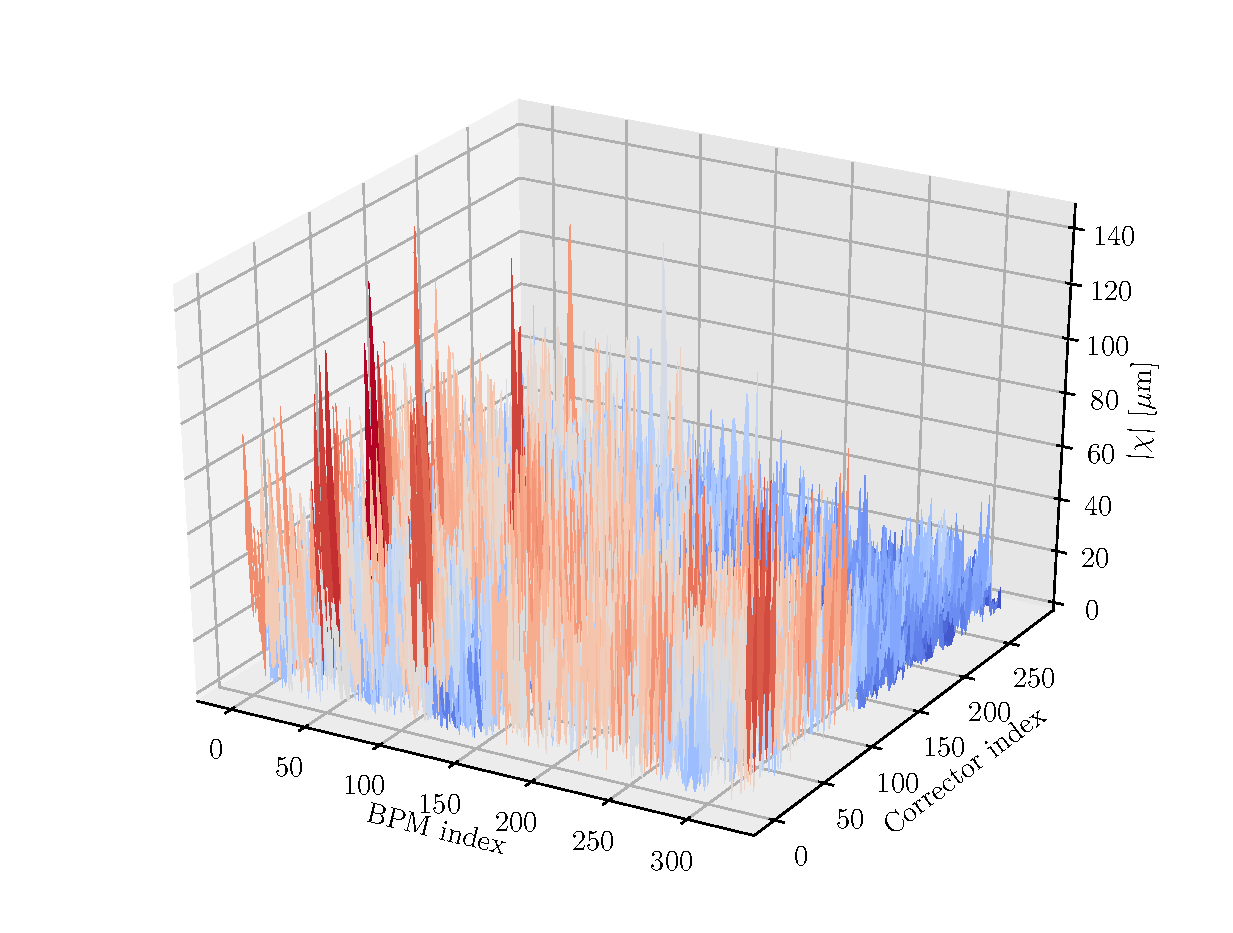
\includegraphics[width=1.0\textwidth]{figures/loco_surface_iter0_before.eps}
%     \caption{Before.}
%     \label{subfig:ondiag}
% \end{subfigure}
%  \begin{subfigure}[t]{0.49\textwidth}
% 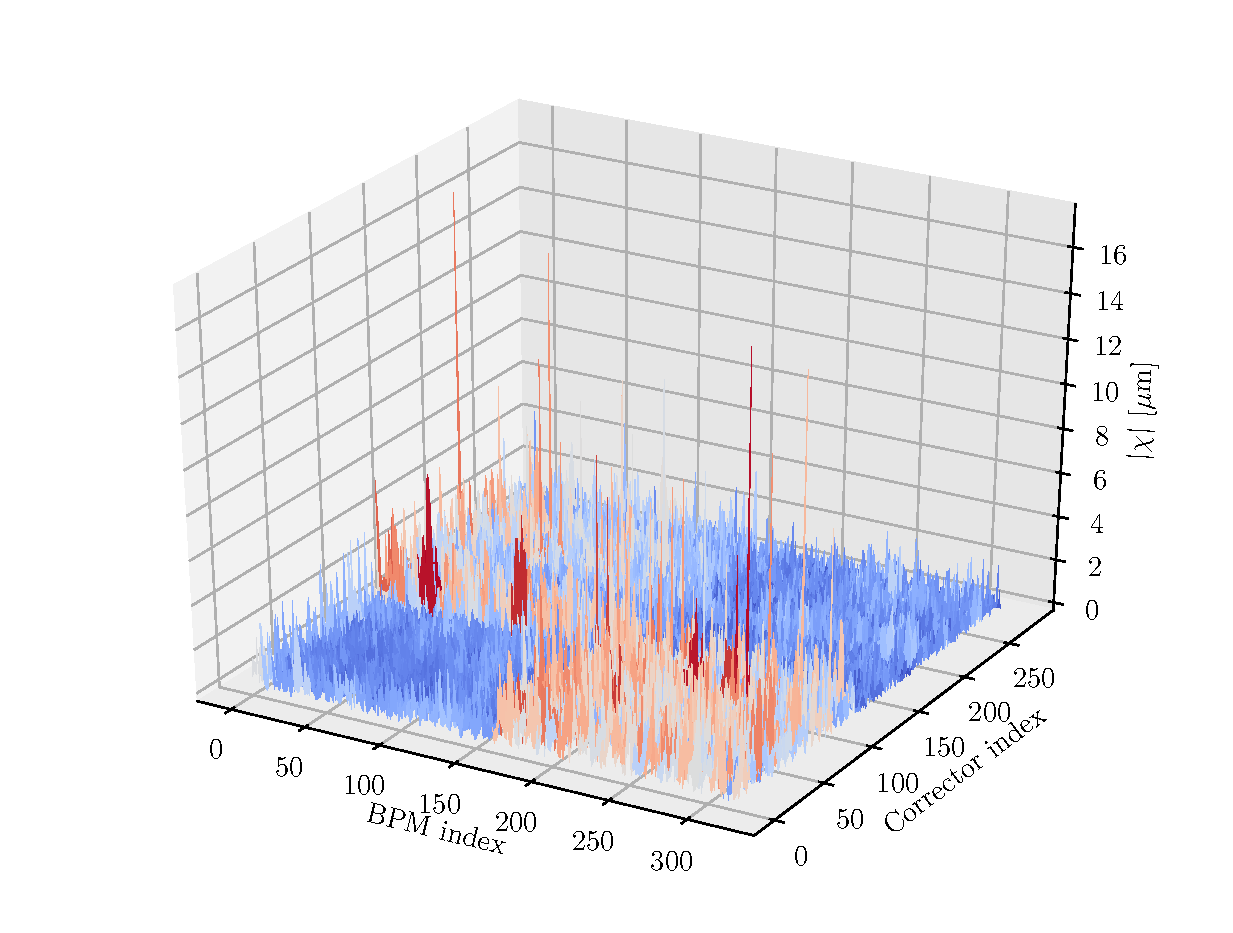
\includegraphics[width=1.0\textwidth]{figures/loco_surface_iter0_after.eps}
%     \caption{After.}
%     \label{subfig:offdiag}
% \end{subfigure}
% \caption{\gls{orm} error distribution before and after LOCO fitting.}
% \label{fig:hist}
% \end{figure}

%The kicks used for conversion are $\Delta \theta_x = \Delta \theta_y = \SI{15}{\micro\meter}$.

% \begin{figure}
% \centering
% \begin{subfigure}[t]{0.49\textwidth}
% 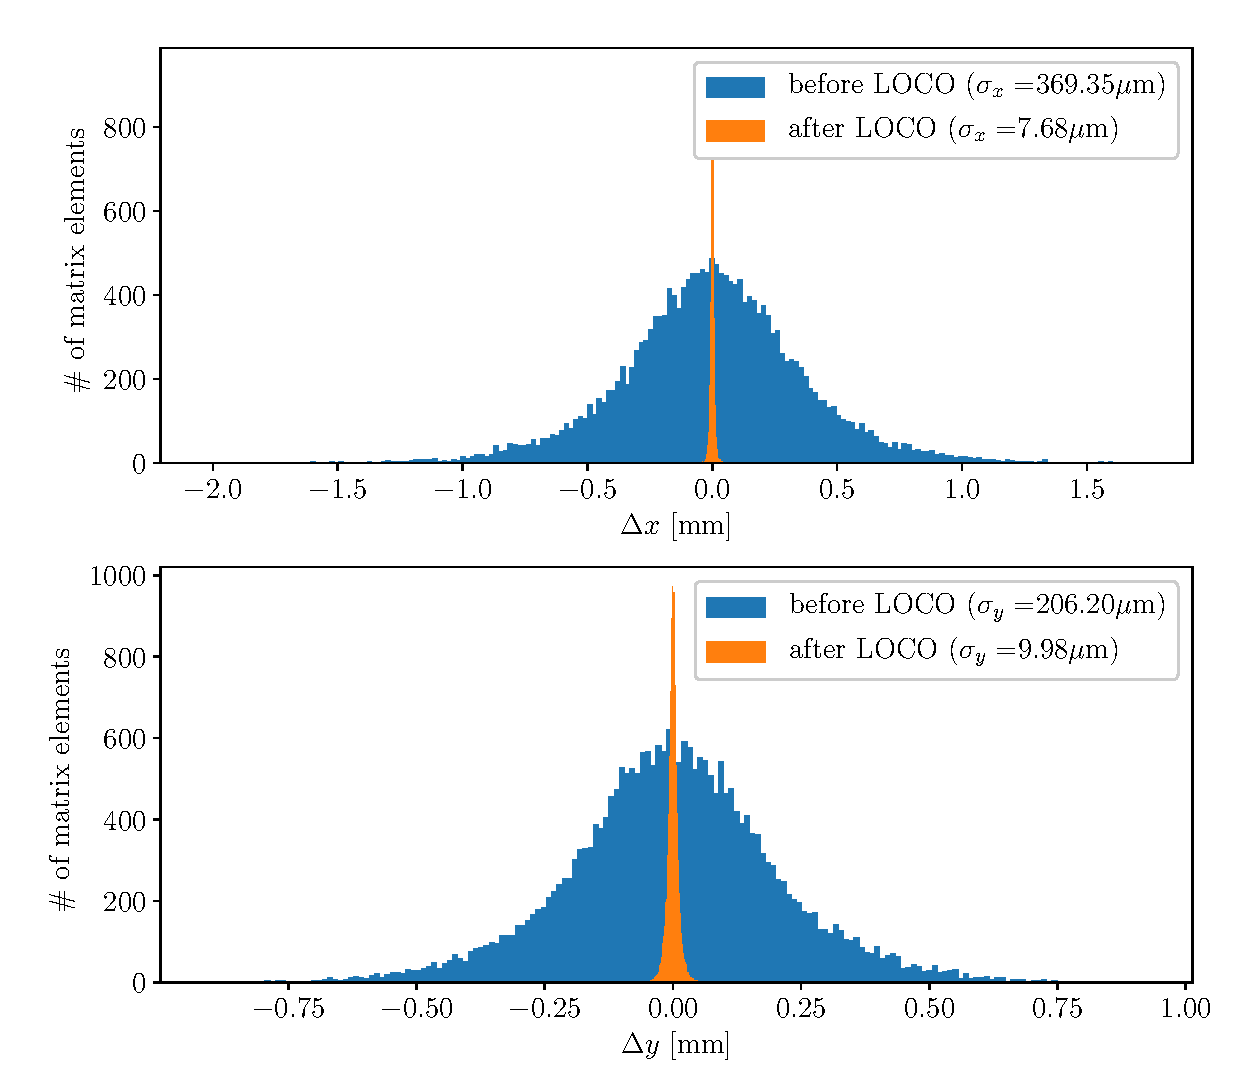
\includegraphics[width=1.0\textwidth]{figures/histogram_iter0_ondiag.eps}
%     \caption{On-diagonal.}
%     \label{subfig:ondiag}
% \end{subfigure}
%  \begin{subfigure}[t]{0.49\textwidth}
% 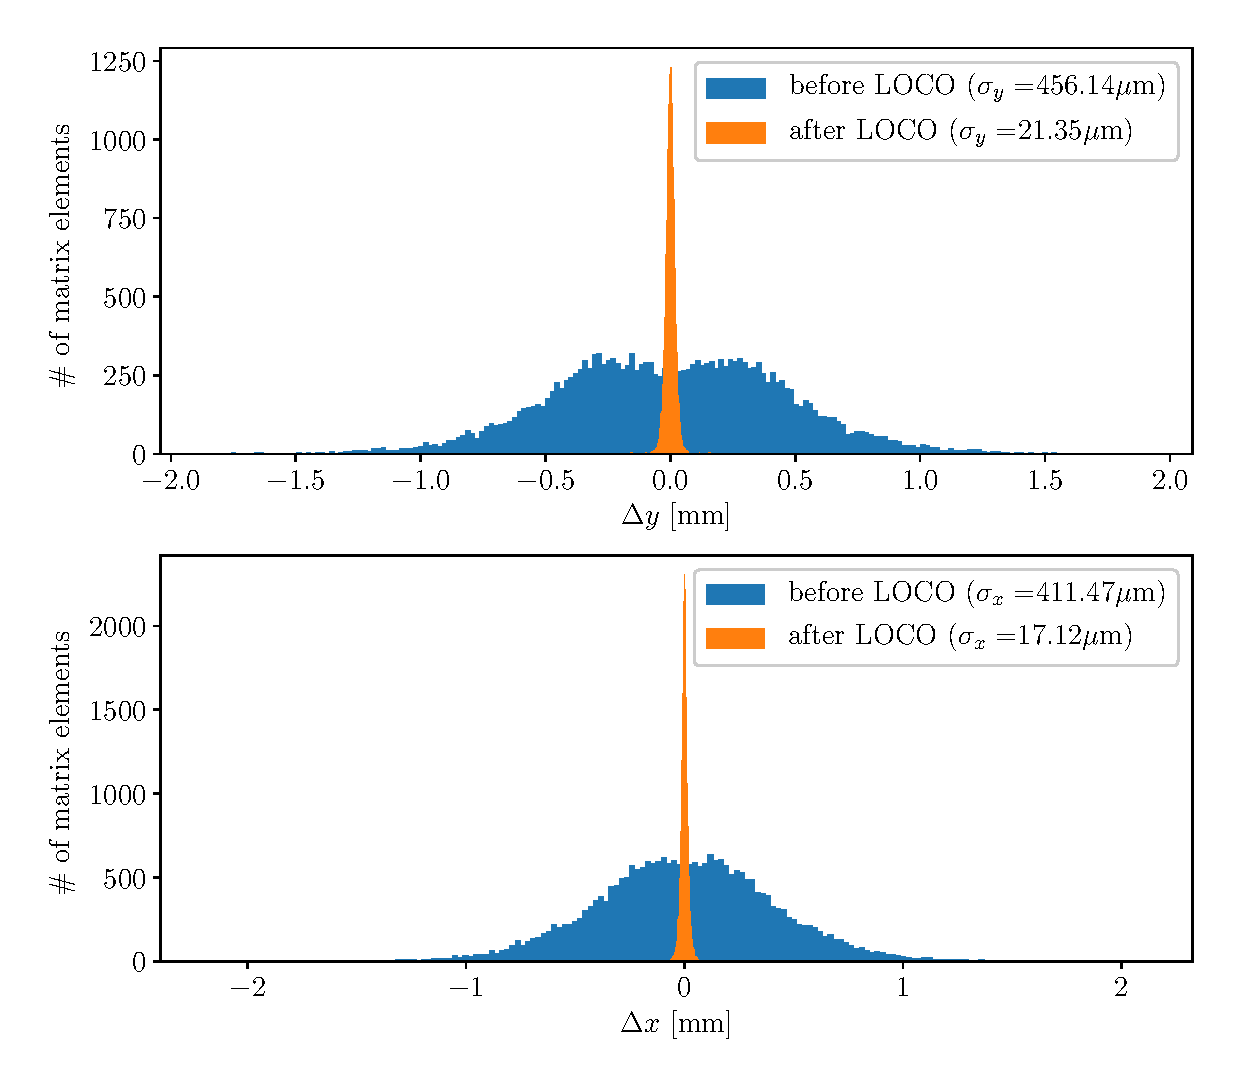
\includegraphics[width=1.0\textwidth]{figures/histogram_iter0_offdiag.eps}
%     \caption{Off-diagonal.}
%     \label{subfig:offdiag}
% \end{subfigure}
% \caption{\gls{orm} error histograms.}
% \label{fig:hist}
% \end{figure}

\section{Tests on Measured Data}
\subsection{Determine the LOCO Configuration}\label{subsec:loco_config}
\subsection{Fit Parameters Variation}
As mentioned in~\cite{safranek1997}: ``\textit{the easiest way to determine how much the set of fit parameters vary due to random errors in the measurements is simply to measure many~\gls{orm}, analyze each one separately, and see how much variation there is between fit parameters for the different data sets}''. Therefore, to determine the variations of fit parameters presented in Table~\ref{tab:fit_params}, the aforementioned procedure was applied in Sirius storage ring, where 10~\glspl{orm} were measured sequentially.

The~\gls{loco} analysis performed in these 10 measured~\glspl{orm} with the configuration described in Subsection~\ref{subsec:loco_config} and the results are organized in Table~\ref{tab:fit_var}.
\begin{table}
    \centering
    \caption{Variations in fit parameters after LOCO analysis of 10 ORM measurements performed in Sirius storage ring.}
    \label{tab:fit_var}
    \begin{tabular}{cccc}
        Parameter & std variation & peak-to-peak variation & Unit \\
        \toprule\toprule
        Quadrupole Relative Strength     & 0.13 & 0.32 & \% \\  
        Skew Quadrupole Absolute Strength& \SI{1.3e-4}{} & \SI{6.2e-4}{} & $\SI{}{\meter^{-1}}$\\
        BPM H. Gain             & 0.06 & 0.27 & \%\\
        BPM V. Gain             & 0.07 & 0.35 & \%\\
        BPM Roll                & 0.25 & 1.31 & $\SI{}{\milli\radian}$ \\
        H. Corrector Gain       & 0.18 & 1.03 & \%\\
        V. Corrector Gain       & 0.21 & 1.14 & \%\\
        \bottomrule\bottomrule
    \end{tabular}
\end{table}
\subsection{Finding Planted Error}
\section{Linear Optics and Coupling Correction}
\section{Independent Measurements}
% \section{Orbit response matrix}
% \section{Transverse Linear Coupling}
% \section{Betatron Function}
% \section{Dispersion Function}
% % \section{Emittance}
% \section{Dynamical Aperture}
% \section{Injection Efficiency}
